\subsection{Bedeutung einer Man-in-the-Middle Attacke}
Man in the Middle (MITM) ist ein Angriffsszenario, bei der ein unberechtigter Dritter versucht, in eine zwischen zwei Kommunikationspartnern geführte, sichere (verschlüsselte) oder auch unsichere (unverschlüsselte) Kommunikation einzudringen. Ziel des Angreifers ist es, die zu übertragenden, vertraulichen Informationen unbemerkt mitzulesen und/oder zu manipulieren. Um unerkannt im Hintergrund an die Daten beziehungsweise Informationen zu gelangen, täuscht der Angreifer vor, der jeweilige andere Kommunikationspartner zu sein. Ein MITM-Angriff kann auf den verschiedenen Ebenen des ISO/OSI Schichten-Modells \cite[vgl.]{osi}, z. B. auf Anwendungsebene (HTTP/HTTPs) oder Netzwerkebene (IP) stattfinden. Quelle: \cite[vgl.]{mitm-def}
\begin{figure}[H]
	\centering
	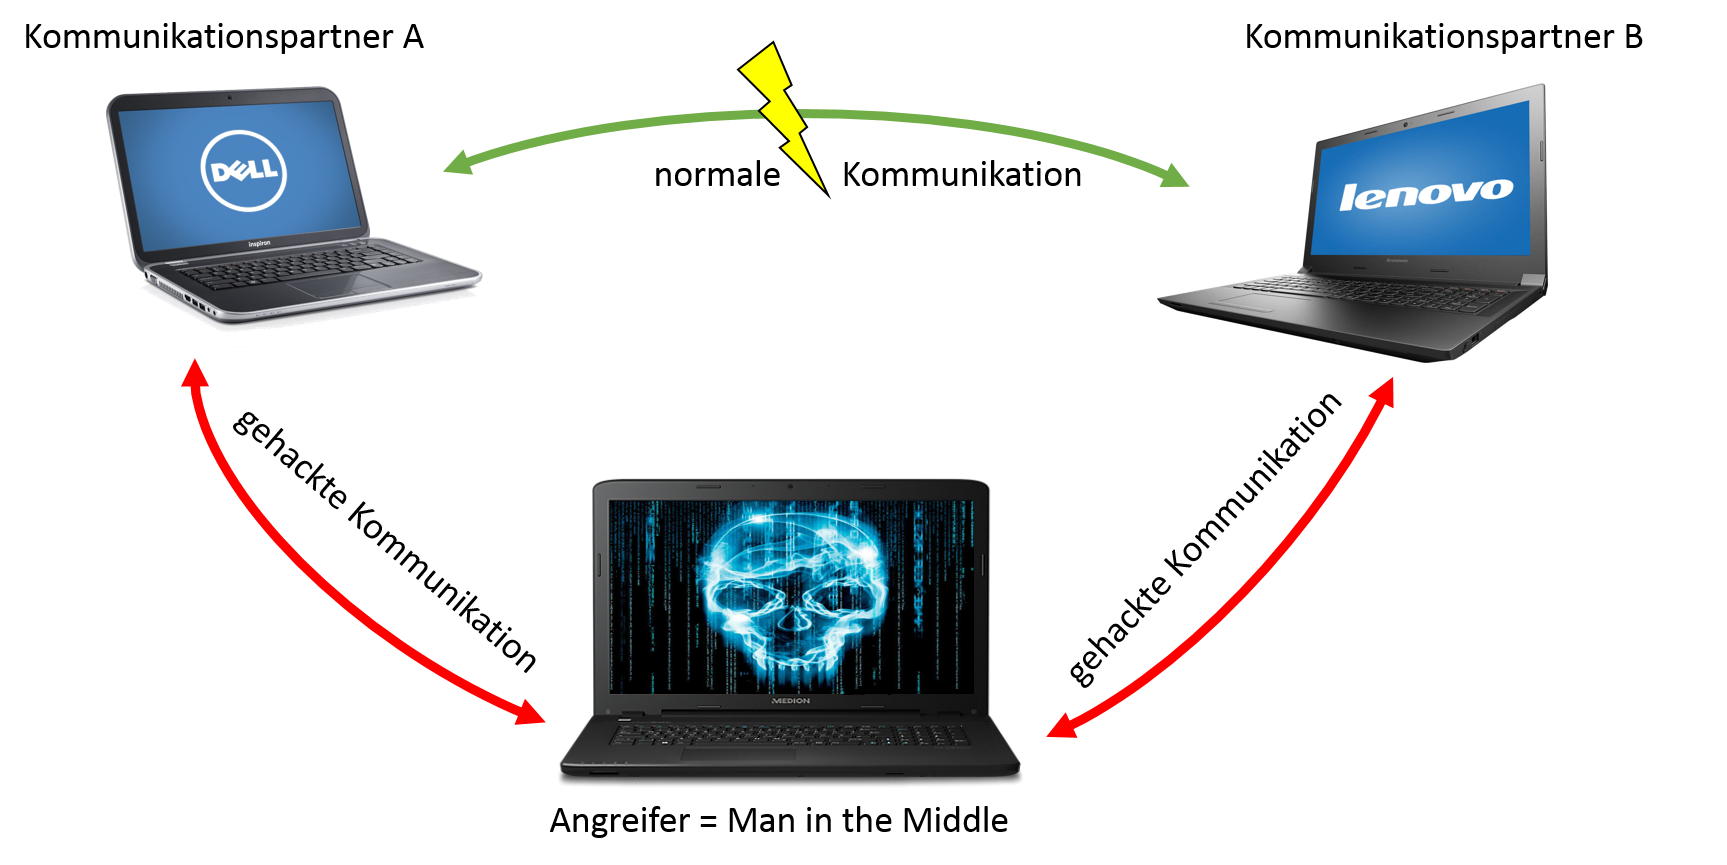
\includegraphics[width=.8\linewidth]{images/MITM.png}
	\caption{Man in the Middle Angriff \cite{mitm-bild}}
\end{figure}